\documentclass[10pt]{beamer}

\usepackage[utf8]{inputenc}
\usepackage{pgfpages}
\usepackage{dirtree}
\setbeameroption{show notes on second screen =left} %hide nodes, show only notes, show notes on second screen = left.
\setbeamertemplate{note page}[plain]
\AtEndNote{\vfill \begin{center} mm:hh \end{center}}
\newcommand{\notedir}[1] {
  \note{\dirtree{#1}}}
\def \ion {$^{\circ}$ }
\usepackage{tcolorbox}
\usepackage{tikz}
\usepackage{tikz-3dplot}
\usetikzlibrary{intersections,calc}
\usepackage{amsmath}
\usepackage{graphicx}
\usepackage{cases}
\def \heart {\textcolor{blue}{$\heartsuit$} }
\def \C {$\mathcal{C}$}
\def \orthog {\underline{\perp}}
\def\arcos{\operatorname{arcos}}

\tcbset{%
	basic/.style={colframe=black,
		      colback=white,
		      top= 0mm,
		      bottom = 2mm,
		      boxsep=0mm
		      }
}

    
\begin{document}  
    \beamertemplatenavigationsymbolsempty
    \setlength{\abovedisplayskip}{0pt}
    \setlength{\belowdisplayskip}{0pt}
    \frame{
	  
	  \frametitle{Q4 Septembre 2001.}
	  On considère un prisme droit $ABCDA'B'C'D'$ , à base carrée $ABCD$ (cf. figure).
	  \renewcommand{\theenumi}{\alph{enumi})}
	  \begin{enumerate}
	   \item Si $X$ est le centre (intersection des diagonales) de la face $A'B'C'D'$, montrez que la hauteur
		 du triangle $BXB'$ issue de $B'$ est perpendiculaire au plan $A'C'B$.
	   \item Prouver que si les diagonales $BD'$ et $B'D$ sont perpendiculaires, alors la
		 perpendiculaire abaissée de $B'$ sur le plan $A'C'B$ passe par le milieu de
		 l’arête $[D,D']$.
	  \end{enumerate}

	  \vfill
	  
	  \pause
	  % hypothèses et thèse
	  \begin{tcolorbox}[basic] 
	      \begin{columns}[t]
		 
		 \column{.5\textwidth}\centering
		      
		      \underline{Hypothèses} 
		      \begin{itemize}
		      \item Prisme droit à base $\square$,
		      \item $B'B_1$ hauteur de $\Delta XBB'$.
		      \end{itemize}

		  
		  \column{.55\textwidth}\centering
		      
		      \underline{Thèse} \\
		      \begin{enumerate}
		       \item $B'B_1\bot A'C'B$,
		       \item $BD'\bot B'D \rightarrow |DB_2|=|B_2D'|$.
		      \end{enumerate} \flushleft
		      {\small $B_1$ pied de la hauteur issue de $B$, \\
			      $B_2=B'B_1\cap DD'.$ }
		     
		
	      \end{columns}
	  \end{tcolorbox}
	  \notedir{%
		  .1 Enoncé.
		  .2 Hypothèses (non visibles sur le dessin)..
		  .2 Thèse : traduction mathématique..
		  .3 $B'$ pied de la hauteur issue de $B$..
		  .3 $B_2$ intersect\ion de la perpendiculaire abaissée et $DD'$..
		  .2 Grand dessin.. 
		  }
    }

    \frame{ 
	  
	  % résolution ex1
	  \begin{columns}[t]
		\column{.56\textwidth}\centering 
		

			\underline{Dessin}\\
			
				  \begin{figure}[h]
				  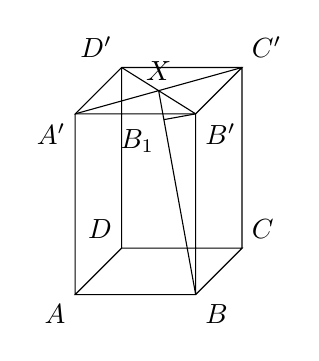
\begin{tikzpicture}[scale=0.765]
				  %AXES
				  %\draw[->] (0,0,-3) -- (0,0,3) coordinate[label=below right:$z$]();
				  %\draw[->] (0,-3,0) -- (0,3,0) coordinate[label=above left:$y$]();
				  %\draw[->] (-3,0,0) -- (3,0,0) coordinate[label=above left:$x$]();	
				  %PRISME DROIT A BASE CARRE
				  \coordinate[label=above left:$D$](D) at (0,0,0);
				  \coordinate[label=above right:$C$](C) at (2,0,0);
				  \coordinate[label=below left:$A$](A) at (0,0,2);
				  \coordinate[label=below right:$B$](B) at (2,0,2);
				  \coordinate[label=above left:$D'$](D') at (0,3,0);
				  \coordinate[label=above right:$C'$](C') at (2,3,0);
				  \coordinate[label=below left:$A'$](A') at (0,3,2);
				  \coordinate[label=below right:$B'$](B') at (2,3,2);
				  
				  \draw (D) -- (A) -- (B) -- (C) --cycle (D') -- (A') -- (B') -- (C') -- cycle					
					(A') -- (A) (D) -- (D') (B') -- (B) (C') -- (C);
				%B',X,B_1	
				\coordinate[label=above:$X$](X) at ($.5*(D')+.5*(B')$);
				\coordinate[label=below left:$B_1$](B_1) at ($(X)!(B')!(B)$);
				\draw   (D') -- (B') (A') -- (C')
					(B') -- (B_1) (B) -- (X);
				  \end{tikzpicture}
				  \end{figure}
			
				  \begin{tcolorbox}[basic] 
				      
				    \smallskip
				    \underline{Hypothèses} 
				    \begin{enumerate}
				    \item Prisme droit à base $\square$,
				    \item $B'B_1$ hauteur de $\Delta XBB'$.
				    \end{enumerate}
							      
				    \underline{Thèse} 
				    \renewcommand{\theenumi}{\alph{enumi})}
				    \begin{enumerate}
				    \item $B'B_1\bot A'C'B$,
				    \item $BD'\bot B'D \rightarrow |DB_2|=|B_2D'|$.
				    \end{enumerate}				    
				    \end{tcolorbox}
		
		
		\column{.5\textwidth}\centering
		
		\underline{Résolution}\\ \flushleft
		
		\heart Une droite est $\bot$ à un plan si elle est ortogonale à 2 droites sécantes de celui-ci.\\ \bigskip
		
		\begin{enumerate}
		 \item $A'C'\bot D'B', A'C'\bot A'A$ \\ \medskip
		       $\rightarrow A'C'\bot XB'B$,\\ \medskip
		       $\rightarrow B'B_1 \orthog A'C'$. \\ \bigskip
		 \item $B'B_1\bot XB$.
		\end{enumerate} \bigskip
		$B'B_1\bot A'C'B$. \hfill $\qed(a)$
	   \end{columns}  
	   \notedir{%
	   .1 Montrer que $B'B_1$ $\bot$ $A'C'B$.
	   .2 Elément de théorie.
	   .3 Droite $\bot$ à plan si $\orthog$ 2 droites sécantes du plan..
	   .2 Résolution.
	   .3 $B'B_1\ \orthog\ A'C'$ car. 
	   .4 $A'C'\ \bot\ DB'B$ car $A'C'\ \bot\ D'B'$ et $\bot\ A'A$.~\\ (Droites $\bot$ plan est $\orthog$ à tt.~droites du plan.).
	   .3 $B'B_1 \bot XB$ car hauteur..
	   .3 $\rightarrow B'B_1 \bot A'C'B$..
	   }
    } 
    \frame{ 
	  \begin{columns}[t]
		\column{.56\textwidth}\centering 
		

			\underline{Dessin}\\
			
				  \begin{figure}[h]
				  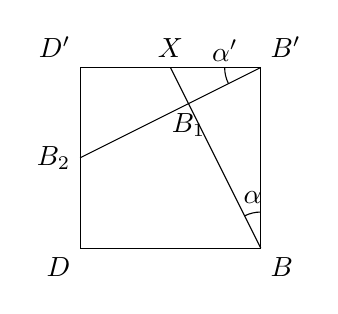
\begin{tikzpicture}[scale=0.765]
				  \coordinate[label=below left:$D$](D) at (0,0);
				  \coordinate[label=below right:$B$](B) at (3,0);
				  \coordinate[label=above right:$B'$](B') at (3,3);
				  \coordinate[label=above left:$D'$](D') at (0,3);
				  \coordinate[label=above:$X$](X) at (1.5,3);
				  \coordinate[label=below:$B_1$](B_1) at ($(X)!(B')!(B)$);
				  \coordinate[label=left:$B_2$](B_2) at (0,1.5);
				  \draw (D) -- (B) -- (B') -- (D') -- cycle;
				  \draw (X) -- (B);
				  \draw (B_2) -- (B');
				  
				  \draw (3,0.6)  arc[radius = 6mm, start angle= 90, end angle= 116.5] node [above,pos=0.5]{$\alpha$};
				  \draw (2.4,3)  arc[radius = 6mm, start angle= 180, end angle= 206.5] node [above,pos=0.2]{$\alpha '$};
				  \end{tikzpicture}
				  \end{figure}
			
				  \begin{tcolorbox}[basic] 
				      
				    \smallskip
				    \underline{Hypothèses} 
				    \begin{enumerate}
				    \item Prisme droit à base $\square$,
				    \item $B'B_1$ hauteur de $\Delta XBB'$.
				    \end{enumerate}
							      
				    \underline{Thèse} 
				    \renewcommand{\theenumi}{\alph{enumi})}
				    \begin{enumerate}
				    \item $B'B_1\bot A'C'B$,
				    \item $BD'\bot B'D \rightarrow |DB_2|=|B_2D'|$.
				    \end{enumerate}				    
				    \end{tcolorbox}
		
		
		\column{.5\textwidth}\flushleft
		$D'B'BD$ carré car les diagonales sont $\bot$. \\ \medskip
		\heart Deux triangles sont isométriques lorsqu'ils ont un côté de même longueur compris entre deux angles de mêmes mesures.\\
		
		\begin{align*}
		|D'B'| =& |BB'|\\[0.5em] 
		\alpha =& \alpha ' \text{ (angles à cotés $\bot$)} \\[0.5em] 
		\widehat{B_2D'B'} =& \widehat{BB'X} = \dfrac{\pi}{2}\\ 
		\end{align*}
		$D'B'B_2, BB'X$ isométriques. \\ \bigskip
		$|DB_2|=|B_2D'|$. \hfill $\qed$
	   \end{columns}  
    \notedir{%
	   .1 Montrer que $BD'\bot B'D \rightarrow |DB_2|=|B_2D'|$.
	   .2 Elément de théorie.
	   .3 Triangles isométriques car égalité de longueurs..
	   .2 Résolution.
	   .3 $D'B'BD$ carré car les diagonales sont $\bot$..
	   .3 2 $\Delta$ sont isométriques si 2 angles et 1 côté égaux..
	   .4 $D'B'B_2, BB'X$ isométriques car.
	   .5 $|D'B'| = |BB'|$ cotés du carré..
	   .5 Chacun un angle droit du carré..
	   .5 $\alpha = \alpha '$ car angles à côtés (carré + thèse a))..
	   .4 $\rightarrow |D'B_2| = |XB'| = $ moitié d'un côté du carré..
	   }
    }
\end{document}
